\documentclass[12pt]{article}
\usepackage{fullpage, braket, amsmath, amssymb}
\usepackage[pdftex]{graphicx}
\usepackage[version=3]{mhchem}
\setlength{\parskip}{5mm}


\begin{document}

\section*{Delayed fluorescence measurements and intensity
  distributions in the frequency domain}

For a pure bright state $\ket{s}$, the normalized fluorescence
intensity is
\begin{equation}
  I_s(t) = \frac{1}{\tau_s} \;
           exp\left[
             -\frac{t}{ \tau_s} 
           \right].
\end{equation}
We consider the case where a pure zero-order bright state is mixed
with a set of $N$ dark states to create a set of $N+1$ mixed states
$\lbrace\ket{m}\rbrace$.  The lifetime of a pure dark state is taken
to be much longer than $\tau_s$.  In this case, the lifetime of a
mixed eigenstate $\ket{m}$ having bright state character $\alpha_m^2$
is
\begin{equation}
  \label{eq:tau-m}
  \tau_m = \tau_s / \alpha_m^2,
\end{equation}
and its intensity is
\begin{equation}
  I_m(t) = \frac{a_m^2}{\tau_s} \;
           exp\left[
             -\frac{a_m^2 \, t}{\tau_s} 
           \right].
\end{equation}
The normalization condition $\sum_m a_m^2 = 1$ leads to the relation
\begin{equation}
  \tau_s^{-1} = \sum_m \tau_m^{-1};
\end{equation}
in this way, $\tau_s$ can be derived from the set of mixed state
lifetimes $\lbrace \tau_m \rbrace$.

We examine the fluorescence intensity after a time delay $\tau_c$,
which we cast in units of the bright state lifetime:
\begin{equation}
  R_c = \tau_c / \tau_s.
\end{equation}
At a multiple $R_c$ of the bright state lifetime, the intensity ratio
between a mixed state and the (hypothetical) pure bright state is
\begin{equation}
  \frac{I_m}{I_s} = a_m^2 \; 
                   exp\left[
                     R_c \, (1 - a_m^2)
                   \right].
\end{equation}
This quantity is in effect a discrimination factor -- it reflects to
what extent the experiment is discriminating in favor of a mixed
eigenstate.  Figure \ref{fig:discr} shows a plot of $I_m/I_s$ for
several values of bright state character.  States with bright
character of 10\% become twice as intense as a pure bright state after
$3\tau_s$.  For a mixed state with 1\% bright character, one must wait
almost $5\tau_s$ before the discrimination factor increases to 1.

\begin{figure}
  \caption{The intensity of a mixed eigenstate relative to the
    intensity of a pure bright state, as a function of time (units of
    bright state lifetime $\tau_s$).  The bright state character is
    varied from 1 to 20 percent.}
  \label{fig:discr}
  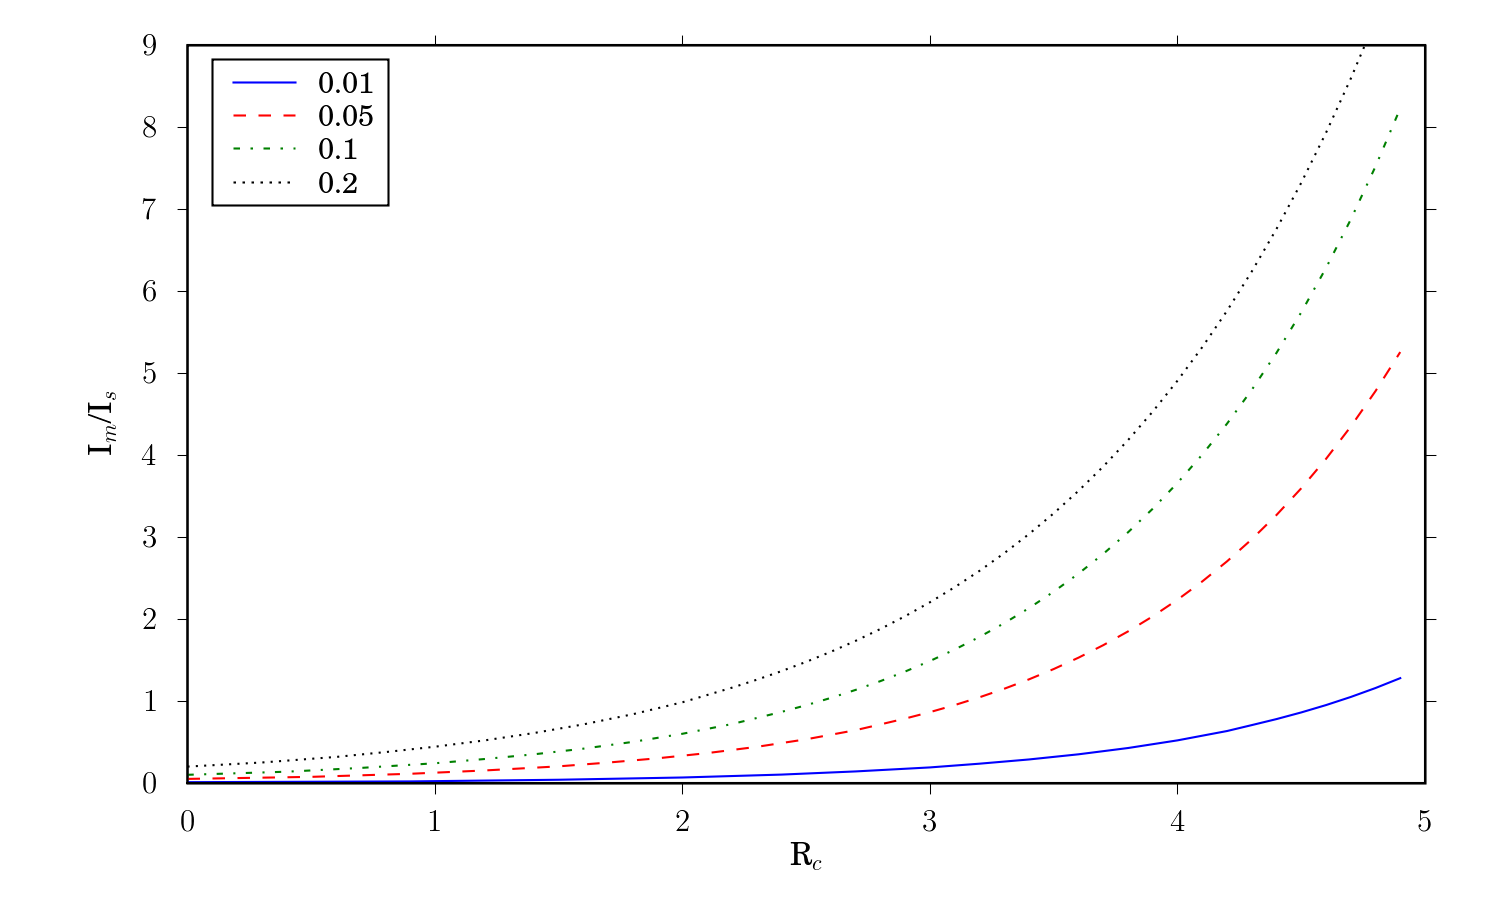
\includegraphics[width=6.5in]{longlife-discrimination.png}
\end{figure}

% Fluorescing states are unobservable in an experiment if the detector
% noise exceeds the fluorescence intensity.  We discuss the noise in an
% experiment as a fraction $f_{\text{noise}}$ of pure bright state
% intensity at $t=0$.  A fluorescing state $\ket{m}$ becomes
% unobservable when
% \begin{equation}
%   I_m(t) = \frac{f_{\text{noise}}}{\tau_s}
% \end{equation}
% The delay time at which any state becomes undetectable is simply a
% function of the bright state character $a_m^2$:
% \begin{equation}
%   (R_c)_{\text{max}} = -\frac{1}{a_m^2} \; 
%                    log\left[
%                      \frac{f_{\text{noise}}}{a_m^2}
%                    \right].
% \end{equation}

We wish to characterize the group of mixed states by their average
fluorescence lifetime $\braket{\tau_m}$.  For the simple case of
direct coupling to a group of evenly spaced levels, the bright state
character follows a Lorentzian distribution in energy.  The width is
given by the golden rule relation
\begin{equation}
  \Gamma = 2 \pi \braket{H_{m}^2} \rho_m.
\end{equation}
The average bright state character, within a constant energy range
$\Delta E$, is proportional to the maximum value of the distribution:
\begin{equation}
  \label{eq:avg-char}
  \braket{a_m^2} \propto \frac{2}{\pi \Gamma} 
                = \frac{1}{\pi^2 \braket{H_{m}^2} \rho_m}.
\end{equation}
The lifetime has an inverse relationship with the bright state
character, so combining equations \ref{eq:avg-char} and \ref{eq:tau-m}
we have
\begin{equation}
  \braket{\tau_m} \propto \tau_s \, \pi^2 \braket{H_{m}^2} \rho_m.
\end{equation}
We have derived, for the simplest case, a proportional relationship
between the average matrix element and average lifetime of a
set of mixed states $\lbrace\ket{m}\rbrace$.

Our next step is to examine the center of gravity of the fluorescence
intensity for a group of lines as we increase the time delay $R_c$.
Consider a system with a single dark state ($N=1$).  The matrix
element 

\end{document}